% This is lnbip.tex the demonstration file of the LaTeX macro package for
% Lecture Notes in Business Information Processing from Springer-Verlag.
% It serves as a template for authors as well.
% version 1.0 for LaTeX2e
%
\documentclass[lnbip]{svmultln}
%
\usepackage{makeidx}  % allows for indexgeneration
% \makeindex          % be prepared for an author index
\usepackage{graphicx}
\usepackage{booktabs}
\usepackage{multirow}
\usepackage{url}
\begin{document}
%
\mainmatter              % start of the contribution
%
\title{Toward Human-Centric Explainable AI: Integrating Large Language Models and Ontologies for Semantically Grounded Explanations}
%
\titlerunning{Human-Centric Ontology-Grounded Explainable AI}  % abbreviated title (for running head)
%                                     also used for the TOC unless
%                                     \toctitle is used
%
\author{Ivar Ekeland\inst{1} \and Roger Temam\inst{2}
Jeffrey Dean \and David Grove \and Craig Chambers \and Kim~B.~Bruce \and
Elsa Bertino}
%
\authorrunning{Ivar Ekeland et al.}   % abbreviated author list (for running head)
%
%%%% list of authors for the TOC (use if author list has to be modified)
\tocauthor{Ivar Ekeland, Roger Temam, Jeffrey Dean, David Grove,
Craig Chambers, Kim B. Bruce, Elisa Bertino}
%
\institute{Princeton University, Princeton NJ 08544, USA,\\
\email{I.Ekeland@princeton.edu},\\ WWW home page:
\texttt{http://users/\homedir iekeland/web/welcome.html}
\and
Universit\'{e} de Paris-Sud,
Laboratoire d'Analyse Num\'{e}rique, B\^{a}timent 425,\\
F-91405 Orsay Cedex, France}

\maketitle              % typeset the title of the contribution

\begin{abstract}
This paper proposes the Human-Centric Ontology-Grounded Explanation (HOGE) framework, which integrates large language models (LLMs) with domain ontologies and knowledge graphs (KGs) to produce semantically grounded, audience-adaptive explanations for machine learning decisions. While Explainable AI (XAI) methods such as SHAP provide valuable technical transparency, their outputs remain difficult for non-technical stakeholders to interpret. LLMs can translate these outputs into natural language but risk hallucination and unfaithful reasoning. HOGE addresses this gap by positioning the ontology as a semantic contract that constrains what explanations can claim, and the LLM as a mediator that translates ontology-grounded evidence into human-consumable narratives. We prototype HOGE in a loan decisioning domain using XGBoost with monotonic constraints, SHAP feature attribution, a Neo4j knowledge graph, and GPT-4o as the narrative explainer. Empirical evaluation across 10~sampled applications demonstrates: average explanation faithfulness of 0.76, semantic fidelity of 0.793, evidence coverage of 0.907, hallucination rate of 20.7\%, perfect graph retrieval accuracy (Precision@K~=~1.0), and 100\% SHAP--prediction alignment. These results demonstrate HOGE's ability to deliver grounded, traceable, and human-readable explanations for high-stakes decisions.
\keywords{Explainable AI, Large Language Models, Ontology, Knowledge Graph, SHAP, Human-Centric AI, Semantic Grounding}
\end{abstract}
%
\section{Introduction}
The deployment of machine learning (ML) and artificial intelligence (AI) systems in real-world settings has outpaced their transition and adaptation by everyday users, particularly due to lack of explanations and assurance methods. In many high-impact domains such as healthcare, public services, cybersecurity, finance, and education; model outputs influence decisions that must be audited and justified to diverse stakeholders with different levels of technical literacy. Explainable AI (XAI) emerged to address this need, providing methods that clarify why a model produced a particular output. However, a persistent issue remains: much of XAI is designed for technical interpretation rather than human understanding. Explanations are frequently produced as feature-attribution scores, saliency heatmaps, or local surrogate models forms that can be valuable to data scientists but difficult for practitioners, auditors, and non-technical decision makers to interpret reliably.
This limitation has been recognized not merely as an engineering inconvenience but as a foundational research challenge: interpretability is not an intrinsic property of a model, but a relationship between an explanation and the audience that consumes it in context~\cite{doshi2017}. If explanation is audience-dependent, then methods optimized primarily for technical audiences risk failing the users who need explanations most. 

Moreover, explanations cannot be created through model outputs in isolation. Decades of research in social science, philosophy, and cognitive psychology show that human explanations tend to be contrastive (``Why outcome A instead of B?''), selective (focusing on a few key causes), and framed in terms of mental models rather than raw statistics~\cite{miller2019}. These properties are frequently absent in typical XAI outputs.

At the same time, recent advances in Large Language Models (LLMs) introduce a new possibility: explanation ``translation''. LLMs can express complex ideas in natural language, adapt tone and detail to an audience, maintain conversational context, and generate structured rationales. Yet LLMs have certain limitations such as hallucination, weak grounding, and inconsistent reasoning especially in domain specific tasks that introduce risks for sensitive applications. A pure LLM-based explanation translation layer can become persuasive rather than faithful to the underlying decision process.

Ontologies and knowledge graphs (KGs) offer a complementary capability for LLMs. Ontologies formally represent domain concepts and relationships, enabling semantic grounding and reasoning. Recent work argues that ontologies can contribute to XAI in multiple roles, including reference modeling (defining what concepts mean), common-sense reasoning (supporting coherent inference over concepts), and knowledge refinement (managing complexity and evolving domain understanding)~\cite{confalonieri2021}. However, ontology-driven explanations are often limited by their usability: logic-based outputs, graph patterns, and formal axioms are rarely communicated in forms that are easily consumable by non-experts.

This paper explores the intersection of these technologies. There is a significant gap remains in the literature: while state-of-art XAI methods provide technical transparency, they often fail to deliver human-centric explanations; while LLMs can generate human-friendly narratives, they require contextual grounding to prevent hallucination and to preserve fidelity; and while ontologies provide semantic structure, they are not typically leveraged as an explanation ``bridge'' to humans. We argue that integrating LLMs with ontological knowledge structures can produce explanations that are (i) semantically grounded, (ii) context-sensitive, and (iii) cognitively aligned to end users, extending impact of traditional XAI to non technical end users.

Key contribution of this paper is a methodologically grounded artifact: a Human-Centric Ontology-Grounded Explanation (HOGE) Framework that uses ontologies to structure context of a AI solution and LLMs to deliver audience-adaptive explanations with explicit grounding. We propose an evaluation approach with metrics that go beyond text similarity to include semantic fidelity, cognitive interpretability, and decision utility, aligning with foundational interpretability evaluation principles~\cite{doshi2017}. We further contribute empirical results from a prototype implementation in loan decisioning, demonstrating explanation faithfulness, grounding precision, and graph retrieval accuracy. The specific research questions addressed are formalised in Section~\ref{sec:gap} following a systematic literature review.

This paper is organised as follows. Section~2 reviews background and related work, identifying the research gap and formulating research questions. Section~3 presents the methodology, Section~4 the proposed HOGE architecture, Section~5 the prototype implementation, Section~6 the evaluation results, and Section~7 the discussion. The paper concludes in Section~8.

\section{Background and Related Work}

This section reviews the three intersecting research streams that underpin HOGE---Explainable AI, Large Language Models for explanation generation, and ontologies/knowledge graphs for semantic grounding---and identifies the research gap and questions that motivate our contribution.

\subsection{Explainable AI: From Technical Transparency to Human Understanding}

XAI has produced a rich toolkit for making ML decisions transparent. Post-hoc feature attribution methods such as SHAP~\cite{lundberg2017} and LIME~\cite{ribeiro2016} have become standard for local model explanation, decomposing predictions into per-feature contributions. More recently, SHAP has been extended through hybrid architectures: Gupta et al.~\cite{dti2025} combined SHAP-based attribution with Kolmogorov--Arnold Networks and LLM-derived protein embeddings for drug--target interaction prediction, producing biologically meaningful explanations of key molecular substructures. Similarly, Alam et al.~\cite{ncd2025} used LLM prompt engineering for domain knowledge extraction and LIME for interpretability in noncommunicable disease prediction, achieving 91.4\% F1-score while revealing actionable socioeconomic determinants.

However, a fundamental limitation persists: XAI methods express explanations as numerical scores, saliency maps, or local approximations that require statistical literacy to interpret. Doshi-Velez and Kim~\cite{doshi2017} argued that interpretability is not an intrinsic model property but a relationship between an explanation and its audience, suggesting that methods optimised for technical audiences risk failing broader stakeholders. Miller~\cite{miller2019} established through comprehensive review of social science literature that human explanations are \emph{contrastive} (``Why X and not Y?''), \emph{selective} (focusing on a few key causes rather than complete causal chains), and \emph{social}---properties largely absent from standard XAI outputs. Bommer et al.~\cite{priork2024} surveyed how prior knowledge including knowledge graphs and cognitive architectures can enhance both robustness and interpretability, concluding that hybrid neuro-symbolic models provide inherent transparency compared to purely post-hoc approaches.

These insights establish a clear need: explanation methods must be designed not only for technical fidelity but also for cognitive alignment with end-user understanding.

\subsection{Large Language Models as Explanation Mediators}

LLMs introduce a powerful capability for XAI: generating fluent, audience-adaptive natural language from structured data. Several recent studies demonstrate this potential across domains.

In cybersecurity, Alsaleem et al.~\cite{ddos2025} combined Random Forest detection with LLM-generated natural language summaries for DDoS attacks, achieving 93\% consistency with human judgement, while Karnati et al.~\cite{klage2026} integrated LIME feature importance into LLM prompts via a Graph-BERT knowledge graph (KLAGE framework) to produce human-readable security reports. In industrial settings, Strahilov et al.~\cite{cip2026} deployed an embedded LLM for conversational diagnostics in a Clean-in-Place system over a six-month field deployment, producing data-grounded explanations from enriched supervisory states while maintaining deterministic safety guarantees.

In healthcare, Khosravi et al.~\cite{medsum2026} introduced MedSumGraph, combining medical knowledge summarisation with GraphRAG and Chain-of-Thought reasoning to produce traceable medical QA responses outperforming domain-specific foundation models. The Chimera-3X system~\cite{chimera2025} orchestrated multiple specialised biomedical LLMs with UMLS and SNOMED CT knowledge graphs, achieving 84\% accuracy on PubMedQA with citation-backed, interpretable answers. Valiauga et al.~\cite{racds2026} demonstrated that a manually curated medical KG integrated with GPT-4o-mini via RAG improved diagnostic reasoning and clinician confidence for rare diseases while reducing hallucinations and enabling selective, trust-calibrated AI adoption.

Despite these advances, LLMs are susceptible to hallucination, particularly when generating claims not grounded in retrieved evidence. Gkournelos et al.~\cite{threat2025} showed that ontology-grounded explanations in the AIThreatTrack system reduced hallucination rates from 47\% to approximately 1.5\% compared to raw GPT-4 outputs in cyber threat hunting, underscoring the importance of structured grounding mechanisms.

\subsection{Ontologies and Knowledge Graphs for Semantic Grounding}

Ontologies formally represent domain concepts, relationships, and constraints, enabling semantic reasoning and structured explanation. Confalonieri et al.~\cite{confalonieri2021} identified multiple roles that ontologies play in XAI, including reference modelling, common-sense reasoning, and knowledge refinement, arguing that ontologies can serve as explanation scaffolds constraining and structuring what AI systems communicate.

Recent work demonstrates ontology-grounded explanation across diverse domains. Jim\'{e}nez-Ruiz et al.~\cite{deibo2025} proposed DEIBO, which explicitly links ontology classes to embedding dimensions in language models, providing white-box-like transparency for otherwise opaque vector representations. In complex system diagnostics, He et al.~\cite{diag2025} encoded functional models as knowledge graphs and used LLM-driven agents to reason over these structures, achieving over 90\% accuracy in element extraction while preserving transparent causal propagation paths.

Knowledge graphs have emerged as critical grounding infrastructure in healthcare. Giannakis et al.~\cite{gdm2026} constructed a Neo4j knowledge graph from 1,212 peer-reviewed articles for gestational diabetes management in a GraphRAG architecture, outperforming ChatGPT, Claude, and BioMistral on clinical relevance metrics. Xu et al.~\cite{synkg2025} proposed a circular joint model where KGs ground LLM reasoning while LLMs continuously expand the KG, achieving accuracy improvements across mental health classification tasks. In education, Sch\"{o}n et al.~\cite{learn2024} showed that KG-contextualised prompts significantly improve the precision and factual accuracy of LLM-generated learning recommendations, while Tsotsolas et al.~\cite{sop2025} used KG-grounded LLMs for explainable SOP chaining and conflict detection in industrial settings.

\subsection{Integrated Approaches: Combining LLMs, KGs, and XAI}

A growing body of work targets the three-way integration of LLMs, KGs, and XAI. In agriculture, Yang et al.~\cite{seeds2025} built SEEDS, a RAG system grounding LLM responses in a pest-control knowledge graph for sustainable farming advisory, while Berrahal et al.~\cite{soil2025} combined soil moisture ML models with the AgriMod ontology and LLMs to produce farmer-friendly semantic explanations. Kumar et al.~\cite{agri2025} developed a multilingual, edge-deployable Digital Twin integrating IoT data with agricultural ontologies and LLMs, achieving 93.1\% advisory accuracy validated by agronomists in rural India.

In medical AI, Zhu et al.~\cite{medkgcot2025} proposed Med-KGCoT, achieving 93.6\% accuracy in medical visual QA through Chain-of-Thought reasoning over dynamically constructed medical KGs. Yang et al.~\cite{depress2025} developed evidence-guided diagnostic reasoning that aligns LLM outputs with a DSM-5 knowledge graph, improving diagnostic accuracy by up to 45\% over direct prompting while enabling claim-level knowledge attribution. Health et al.~\cite{cognet2025} proposed COGNET-MD-X-REQ, an OSCE-inspired evaluation framework using KGs and NER to identify specific LLM weaknesses in multimodal medical diagnosis, keeping clinicians in the loop for curating targeted fine-tuning data.

In e-government, Kouroupetroglou et al.~\cite{egov2025} proposed a hybrid multi-agent GraphRAG architecture with cross-agent verification for policy-compliant question answering, reducing hallucinations through structured reasoning over policy knowledge graphs. Singh et al.~\cite{hybridkg2025} investigated hybrid LLM--KG integration using embedding alignment and contextual fusion, demonstrating improvements in contextual accuracy, entity disambiguation, and explainability through ontology-grounded reasoning paths. The COMPASS framework~\cite{compass2025} augmented LLMs with movie knowledge graphs for explainable conversational recommendations, showing that KG-grounded reasoning outperforms even GPT-4o in recommendation quality and explanation factual consistency.

In broader surveys, Alonso Alemany et al.~\cite{macds2026} systematically reviewed 42 studies combining multi-agent RL, ontologies, and LLMs for clinical decision support, concluding that this combination creates the strongest foundation for adaptive, transparent systems---yet identified a significant lack of real-world validation. De La Cruz Mart\'{i}nez et al.~\cite{pipe2024} positioned LLMs as unifying interfaces for data pipelines, identifying strong synergies with KGs for grounding and with XAI for generating human-understandable explanations, while noting fundamental technical and ethical challenges.

\subsection{Research Gap and Research Questions}
\label{sec:gap}

Despite the breadth of work at the intersection of XAI, LLMs, and ontologies/KGs, our systematic analysis of the literature reveals five persistent gaps:

\begin{enumerate}
    \item \textbf{No semantic contract architecture.} Existing approaches use ontologies for retrieval or reasoning, but none formally position the ontology as a \emph{semantic contract} that constrains what LLM-generated explanations are allowed to claim. Most KG--LLM integrations focus on augmenting LLM accuracy rather than governing explanation validity~\cite{synkg2025,hybridkg2025}.

    \item \textbf{Incomplete explanation pipelines.} Systems typically address one or two stages (e.g., KG retrieval + LLM generation) but lack an end-to-end pipeline from ML prediction through feature attribution, ontology-grounded evidence assembly, policy rule evaluation, and constrained narrative generation with full provenance~\cite{threat2025,sop2025}.

    \item \textbf{Evaluation beyond text similarity.} Most integrated systems report BLEU, ROUGE, or BERTScore~\cite{gdm2026,medsum2026,medkgcot2025}, which measure linguistic quality but not semantic fidelity to the underlying model or domain constraints. Evaluations rarely include perturbation-based faithfulness testing, hallucination characterisation under ontological constraints, or graph retrieval precision.

    \item \textbf{Limited human-centric design grounding.} While many systems claim human-centricity, few operationalise the social science insights of Miller~\cite{miller2019} that explanations should be \emph{contrastive}, \emph{selective}, and \emph{context-appropriate}. Evaluation frameworks rarely measure whether explanations improve actual comprehension, trust calibration, or decision utility~\cite{doshi2017,racds2026}.

    \item \textbf{Domain-agnostic reusability.} Most frameworks are tightly coupled to a single domain (clinical, cybersecurity, agriculture), with limited discussion of how the architecture could be instantiated across domains through a generic ontology contract~\cite{macds2026}.
\end{enumerate}

Based on these gaps, we formulate the following research questions:

\noindent\textbf{RQ1:} How can an ontology serve as a semantic contract that constrains LLM-generated explanations to only reference grounded evidence, and what is the resulting impact on hallucination rate?

\noindent\textbf{RQ2:} To what extent do ontology-grounded LLM explanations faithfully reflect the underlying ML model's reasoning, as measured through perturbation-based faithfulness testing?

\noindent\textbf{RQ3:} Can a knowledge graph-based evidence pipeline preserve complete explanation provenance and achieve lossless retrieval accuracy for feature attributions and policy rules?

\section{Methodology}
\subsection{Design Science Research Methodology}

We adopt the Design Science Research Methodology (DSRM) to guide the development of the proposed HOGE framework. DSRM is well suited for this research as we to create and evaluate an artifact designed to solve a practical problem and contribute knowledge to the field~\cite{peffers2007}. In information systems and socio-technical domains, design science emphasizes building artifacts that address the interplay between people, organizations, and technology~\cite{hevner2004}. Because the core motivation of this work is human-centered explainability; an inherently socio-technical goal DSRM provides a methodologically appropriate structure for us.

DSRM includes multiple stages- problem identification and motivation, objectives of a solution, design and development, demonstration, evaluation, and communication~\cite{peffers2007}. Hevner et al.~\cite{hevner2004} emphasises that design science should produce innovative artifacts and evaluate them rigorously within a relevant environment. Following sections discuss how each stage is applied to this research.

\subsection{Stage 1- Problem Identification and Motivation}
As discussed in Section~1 and~2, during DSRM Stage~1- problem identification and motivation, we identified that many real world ML-based decision systems such as loan approvals and fraud detection produce predictions that are:
\begin{itemize}
    \item hard to explain to non-technical end users
    \item difficult to justify against business policies
    \item sourced from data fragmented across systems (e.g. ML model input features are stored in one database, validation rules are scripted into another system)
    \item not reusable across applications (e.g. across different products of same organisation such as loan and insurance through a bank)
\end{itemize}

Yet the regulated decisions such as home loan approvals needs explanations that are:
\begin{itemize}
    \item faithful (match model behavior)
    \item actionable (what can end-user do to change decision outcome)
    \item policy-aware (connect model reasons to business constraints)
    \item auditable (traceable provenance).
\end{itemize}
The key gap we identified is lack of a unified representation layer that ties together prediction, feature evidence, explanations, rules, and produce human-readable narratives.

\subsection{Stage 2 --- Define Objectives for a Solution}
Based on the Stage~1, we define our solution objectives as:
\begin{itemize}
    \item \textbf{Unified representation}--- Store prediction + feature values + SHAP contributions + policy rules in a single graph.
    \item \textbf{Explainability completeness}--- For a given application, retrieve: prediction, probability, top drivers, and violated rules.
    \item \textbf{Human interpretability}--- Generate a consistent narrative explanation (template + optional LLM verbalizer).
    \item \textbf{Auditability}--- Persist provenance (model version, data timestamp, loader version).
    \item \textbf{Reusability}--- Solution can be used with any dataset/model/explanation method outputs through a generic contract (domain-agnostic core with standardised input/output formats).
    \item \textbf{Extensibility}--- Add new ML models, XAI methods and evaluation metrics without redesigning the graph.
\end{itemize}

\subsection{Stage 3 - Design and Development}

Based on the objectives identified in Stage~2, the artifact we design and develop is a conceptual and architectural framework for human-centric explanations at the intersection of XAI, LLMs, and ontologies. 
We propose a framework termed Human-Centric Ontology-Grounded Explanation (HOGE). HOGE is not ``just'' an LLM interface for an XAI method, nor ``just'' an ontology attached to a model. Instead, HOGE treats the ontology as a semantic contract that shapes what explanations can say, and treats the LLM as a mediator that translates ontology-grounded evidence into human-consumable narratives.


\subsection{Stage 4 - Demonstration}
Its evaluation is operationalized via a use case and a proposed metric suite and an experimental plan aligned with interpretability evaluation guidance~\cite{doshi2017}.

\subsection{Stage 5- Evaluation}

\begin{figure}[htp]
    \centering
    \includegraphics[width=\linewidth]{HOGE_Evaluation_Framework.pdf}
    \caption{Evaluation framework}
    \label{fig:evalFramework}
\end{figure}


A central weakness in the current literature is that evaluation of explanation quality is often reduced to proxy metrics. For example, RAG/GraphRAG systems frequently report BLEU/ROUGE/BERTScore and related similarity metrics, which can correlate with linguistic quality but do not guarantee human usefulness. In clinical decision support settings, human-centered evaluation is increasingly emphasized because explanation usefulness must relate to decision-making outcomes rather than language fluency alone~\cite{doshi2017}.

We evaluate HOGE across three levels, grounded in interpretability evaluation taxonomy~\cite{doshi2017} and illustrated in Figure~\ref{fig:evalFramework}. These levels collectively operationalize the human-centered view that explanation value is measured by usefulness in context~\cite{doshi2017,miller2019}.

\subsection{Level 1: Semantic and Factual Grounding (Functionally Grounded Evaluation)}
This level tests whether explanations remain consistent with ontology constraints and retrieved evidence. Proposed metrics include:

\begin{itemize}
    \item \textbf{Semantic Fidelity (SF)}: the proportion of explanation claims that map to ontology concepts and relations without violating constraints~\cite{confalonieri2021}.
    \item \textbf{Evidence Coverage (EC)}: the proportion of claims backed by explicit evidence bundles (KG paths, retrieved passages, provenance).
    \item \textbf{Hallucination Rate under Constraint (HRC)}: rate of unsupported claims when ontology + evidence constraints are enforced.
\end{itemize}

\subsection{Level 2: Human Comprehension and Trust Calibration (Human-Grounded Evaluation)}
This level uses controlled user studies with simplified tasks, measuring comprehension and calibrated trust:
\begin{itemize}
    \item \textbf{Comprehension Score (CS)}: accuracy on questions testing understanding of why a prediction occurred and what would change it.
    \item \textbf{Trust Calibration Error (TCE)}: difference between user confidence and model reliability, indicating over-trust or under-trust.
\end{itemize}
These align with the argument that interpretability is audience-relative and must be evaluated with humans~\cite{doshi2017,miller2019}.

\subsection{Level 3: Real-World Decision Utility (Application-Grounded Evaluation)}
This level evaluates whether explanations improve real task performance:
\begin{itemize}
    \item \textbf{Decision Utility Gain (DUG)}: improvement in decision accuracy or speed compared to baseline XAI outputs.
    \item \textbf{Actionability Index (AIx)}: proportion of explanations that lead to correct recommended actions, aligned to domain goals.
\end{itemize}


\subsection{Stage 6- Communication}



\section{Proposed HOGE Architecture}

The HOGE system architecture consists of three major components: predictive modelling and technical explainer, semantic knowledge representation, and narrative explanation. Figure~\ref{fig:architecture} presents the high-level architecture of the HOGE framework, illustrating the data flow from the predictive model through the semantic knowledge layer to the narrative explainer.

\begin{figure}[htp]
    \centering
    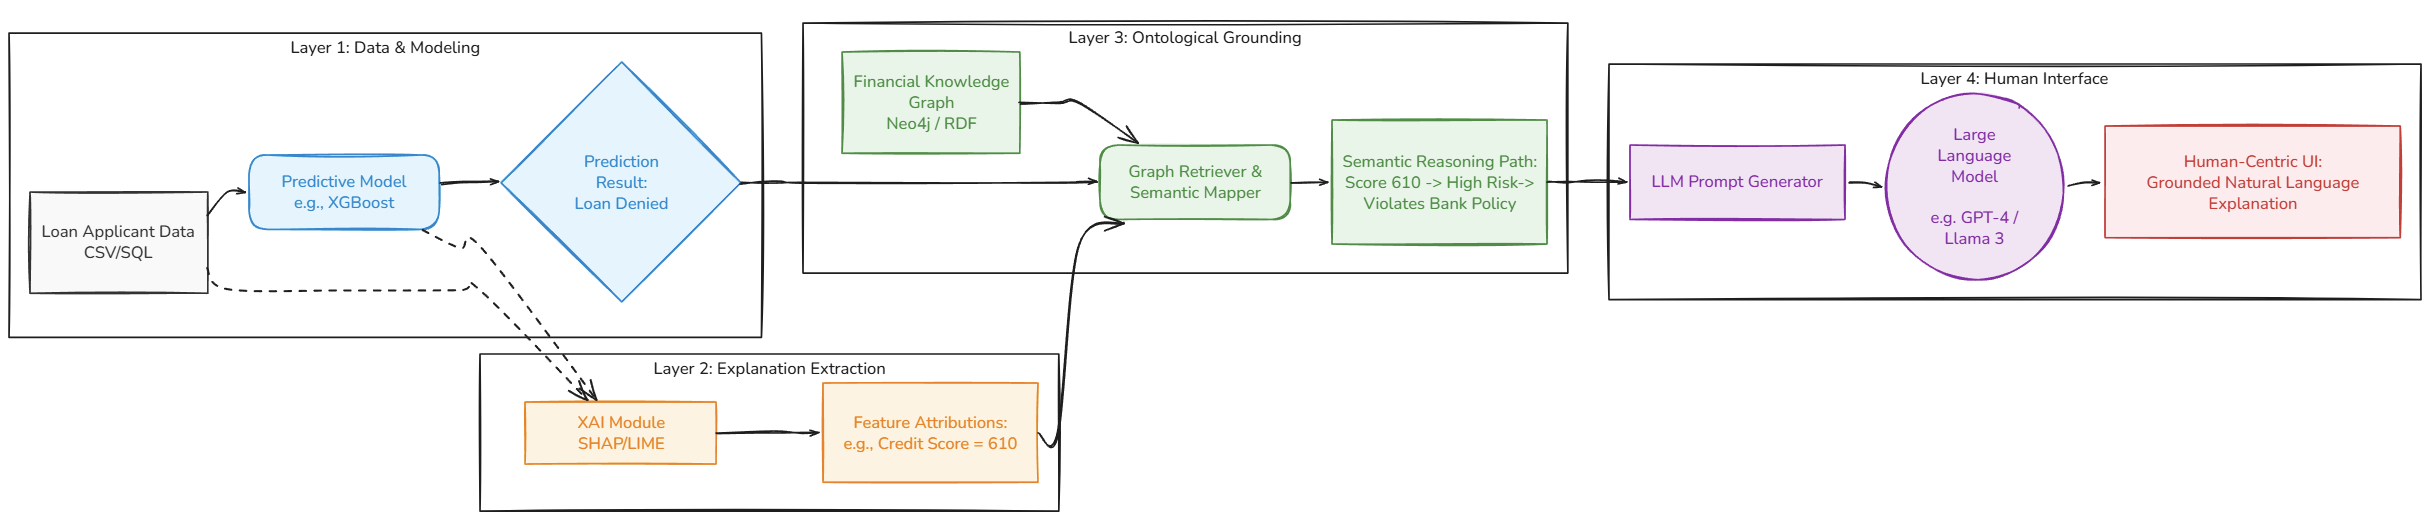
\includegraphics[width=\linewidth]{Architecture.png}
    \caption{HOGE system architecture: Component~A (Predictive Model and Technical Explainers), Component~B (Semantic Knowledge Representation), and Component~C (Narrative Explainer) interact to produce human-centric, ontology-grounded explanations.}
    \label{fig:architecture}
\end{figure}

\subsection{Component A: Predictive Model and Technical Explainers}

HOGE is designed to integrate into existing predictive models and model explainability methods. For example, explainability methods may include feature attribution (e.g., SHAP~\cite{lundberg2017}), local surrogate models (e.g., LIME~\cite{ribeiro2016}), counterfactual generation, and uncertainty estimation. HOGE does not replace technical XAI, but extend its capability.

\subsection{Component B: Semantic Knowledge Representation}
This component contains an ontology (schema) and a knowledge graph (KG) and support reasoning and traceability, consistent with the roles of ontologies in XAI described by Confalonieri and Guizzardi~\cite{confalonieri2021}.
The ontology defines domain concepts, relationships, constraints, and permissible explanation primitives. For example, in the context of cybersecurity, the ontology may define threat categories, behaviors, assets, vulnerabilities, and response actions. In agriculture, the ontology defines irrigation concepts and soil states, enabling explanations aligned to farmer cognition. 

We ground the HOGE ontology on RVO model and extend to capture unified representation necessary to support end-user friendly explanations. The main classes and relationships of HOGE ontology are represented in Figure~\ref{fig:HOGEontology}.

\begin{figure}
    \centering
    \includegraphics[width=\linewidth]{HUGO-OntologyV1.pdf}
    \caption{The ontology for HOGE}
    \label{fig:HOGEontology}
\end{figure}

Figure~\ref{fig:kg_schema} shows the instantiated ontology schema as realised in the Neo4j knowledge graph, depicting the eight node labels (Applicant, LoanApplication, Feature, FeatureValue, ModelExplanation, FeatureContribution, PolicyRule, RiskFactor) and their directed relationship types.

\begin{figure}[htp]
    \centering
    
\includegraphics[width=\linewidth]{neo4j_kg_schema.png}
    \caption{HOGE Knowledge Graph --- ontology schema view extracted from Neo4j, showing node labels and relationship types.}
    \label{fig:kg_schema}
\end{figure}

To create an associated knowledge graph from the ontology, we use an ingestion pipeline:
\begin{enumerate}
    \item Creates constraints (uniqueness on application IDs, feature names, explanation IDs)
    \item Loads application-level nodes (Applicant, LoanApplication, demographic attributes)
    \item Loads SHAP explanation nodes + contribution nodes (signed values, absolute importance, rank, direction)
    \item Loads feature values and links them via feature name
    \item Loads policy rules and risk factors, then links violations to applications
\end{enumerate}

Each evidence item is persisted with an explicit KG path (e.g., \texttt{(LoanApplication:LP001006) -[:HAS\_SHAP\_EXPLANATION]-> (ModelExplanation) -[:HAS\_CONTRIBUTION]-> (FeatureContribution) -[:FOR\_FEATURE]-> (Feature:CoapplicantIncome)}), enabling full provenance traceability from any narrative claim back to its source in the graph.

Figure~\ref{fig:kg_instance} shows the instance-level subgraph for loan application LP001006, illustrating how a single application node connects to its applicant, feature values, SHAP contributions, and feature definitions through the relationships defined in the ontology schema.

\begin{figure}[htp]
    \centering
    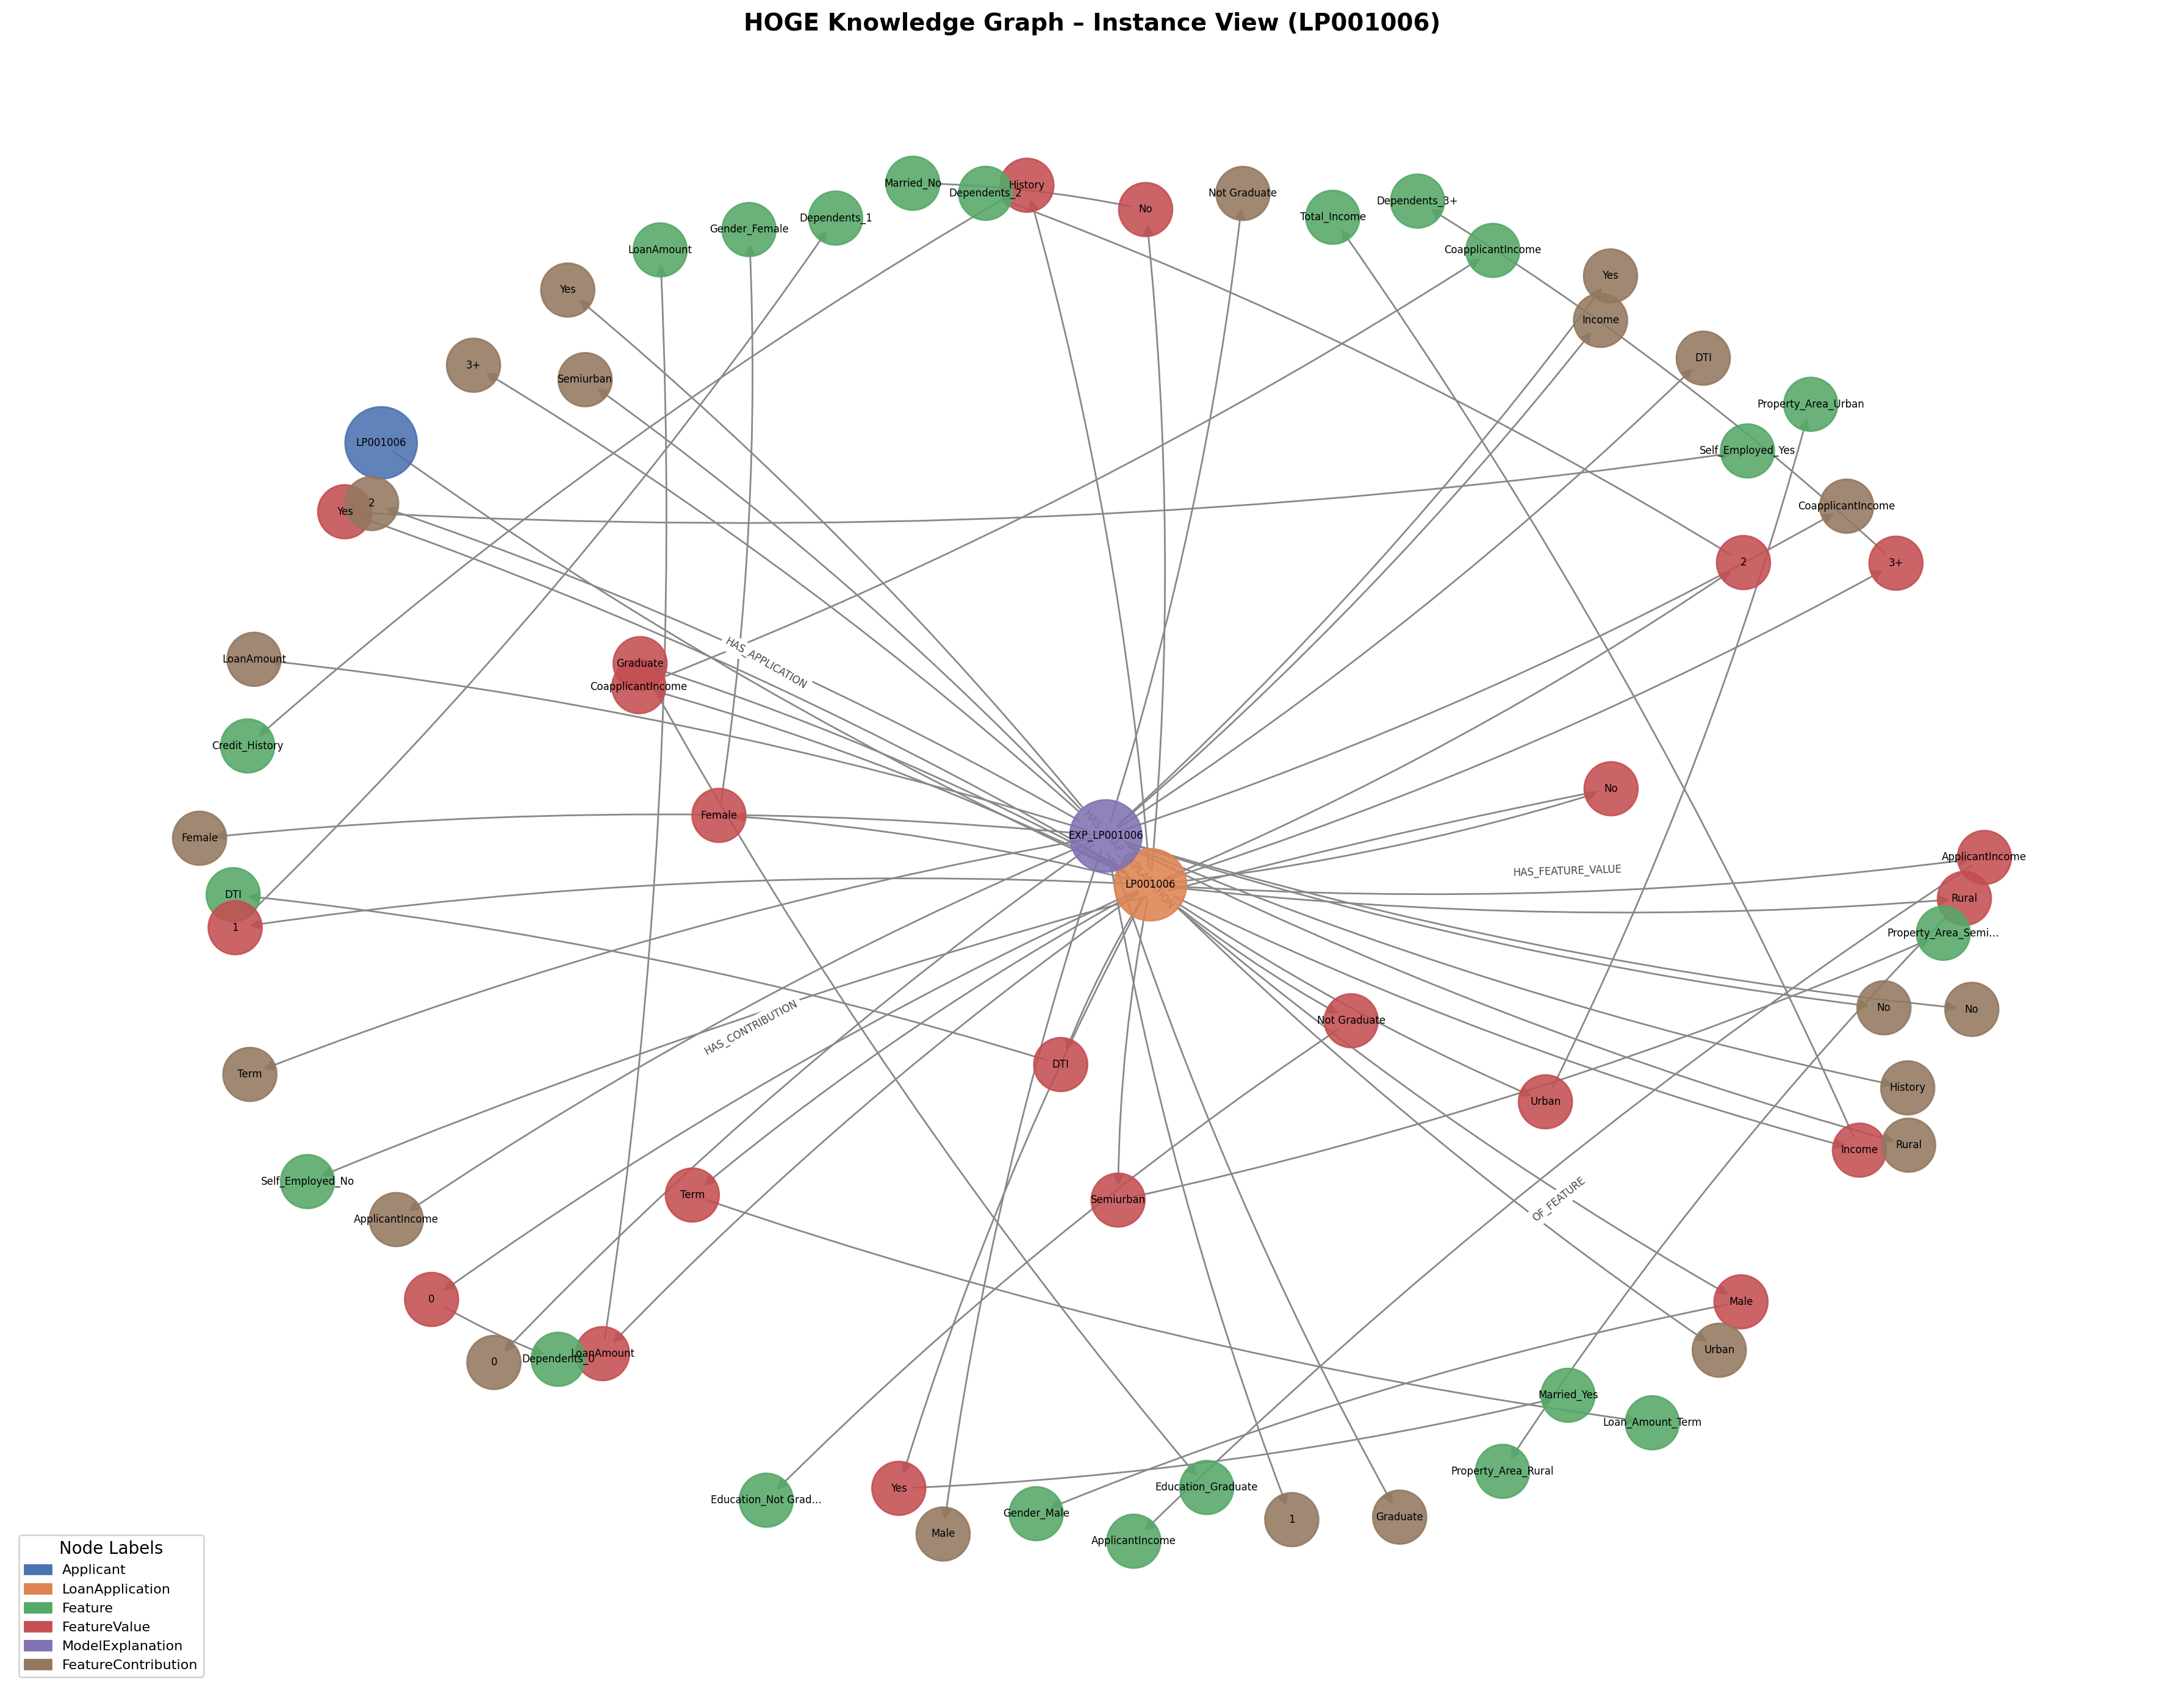
\includegraphics[width=\linewidth]{neo4j_kg_instance.png}
    \caption{Knowledge graph instance view for application LP001006, showing the full subgraph of applicant profile, feature values, SHAP feature contributions, and model explanation nodes.}
    \label{fig:kg_instance}
\end{figure}


\subsection{Component C: Narrative Explainer}
The role of Narrative Explainer is to generate explanations in natural language only operating within the concepts and claims provided through semantic knowledge representation layer. 
Its key function is to turn concept-evidence pairs into coherent narratives aligned with how humans understand explanations (contrastive, selective, and context-appropriate)~\cite{miller2019}.

The Narrative Explainer operates under strict grounding constraints. The LLM prompt is constructed to include:
\begin{itemize}
    \item ALL feature contributions ranked by importance (the complete evidence set)
    \item ALL known policy rules from the domain ontology (the semantic contract)
    \item Explicit instructions that the LLM must ONLY reference features and rules present in the evidence
    \item A structured JSON output format requiring: summary, positive drivers, negative drivers, policy violations, recommendation, full narrative, and a list of features used
\end{itemize}

This structured output enables automated evaluation. The final working query produces a structured response that contains:
\begin{itemize}
    \item prediction + its probability
    \item Model explanation details (feature, value, importance, rank, direction)
    \item violated rules list (rule\_id, description, severity)
    \item evidence bundle: KG paths backing each claim
    \item provenance metadata (model version, XAI method, KG loader version, timestamp)
\end{itemize}

    
\subsection{User Interface Integration}
We propose to deliver the ML outcome and explanations to end user through an interface that supports iterative questioning, progressive disclosure (from high-level summary to deeper detail), and loop in the user feedback. This design is based on human-centered XAI design literature~\cite{miller2019} suggests such interaction patterns are essential, because explanation needs evolve as users explore the model's decision.

LLM explainer is connected to the user interface through an API endpoint.
API endpoint accepts the case details (e.g.id) form the user, invoke ML model and technical explainer and query the KG for unified details of ML outcome. This will be provided as a structured JSON that is converted into human-readable explanation through LLM Explainer and return to the user.


\section{Prototype Implementation}

\subsection{Case Study Overview}
For demonstration of the utility of HOGE, we prototype an end-to-end Explainable AI (XAI) pipeline for loan decisioning, integrating monotonic gradient boosting as ML models, local feature attribution with SHAP, and a finance domain aware Knowledge Graph (KG) to generate context-rich, human-centric explanations. The prototype uses the publicly available Loan Eligible Dataset from Kaggle~\cite{kaggle_loan}, which contains 614~loan application records with demographic, financial, and credit attributes.

We demonstrate how HOGE performs over three scenarios:
\begin{itemize}
    \item \textbf{Scenario~1}: End user provides a loan application ID (e.g. LP001006). HOGE Output: prediction, probability, top SHAP drivers, linked feature values.
    \item \textbf{Scenario~2}: Explanation narrative generation for top positive/negative drivers. HOGE Output: natural language explanation using structured prompt through LLM, returned as JSON with summary, drivers, violations, recommendation, and full narrative.
    \item \textbf{Scenario~3}: Policy validation for a given application ID. HOGE Output: rules violated (if any), severity, linked risk factors, and KG provenance paths.
\end{itemize}


\subsection{Predictive Model}
A gradient boosting model (XGBoost) with domain constraints was trained on the Loan Eligible Dataset~\cite{kaggle_loan}, a publicly available structured financial dataset containing 614~loan application records. After pre-processing (removing incomplete records and engineering derived features such as TotalIncome and Debt-to-Income ratio), 500~applications were retained for model training and evaluation. The pre-processed features used for model training include:
\begin{itemize}
    \item Income features (ApplicantIncome, CoapplicantIncome, TotalIncome)
    \item Credit history
    \item Loan amount and tenure
    \item Debt-to-Income ratio (DTI)
    \item Encoded categorical variables (Property Area, Gender, Dependents, Education, etc.)
\end{itemize}

Following monotonic constraints were incorporated to enforce domain logic:
    \begin{itemize}
        \item increasing income should not reduce approval probability;
        \item increasing debt-to-income ratio (DTI) should not increase approval probability;
        \item improving credit history should never worsen the predicted risk.
    \end{itemize}
This guarantees that the model adheres to common lending logic and ensures regulator-compliant model behaviour by eliminating counterintuitive patterns.

The trained model achieved an ROC-AUC of 0.839 on the held-out test set (20\% split, stratified), with precision of 0.88 for approved applications and 0.66 for declined applications, yielding an overall accuracy of 80\%. The model produced a probabilistic approval score for each of the 500~applications.


\subsection{Technical Explainer}
As the XAI method, we utilised Tree SHAP algorithms to explain the output of the XGBoost model. SHAP TreeExplainer captured the marginal contribution of each of the 22~transformed features to each loan outcome, producing:
\begin{itemize}
    \item Signed SHAP contribution (positive $\rightarrow$ increases approval; negative $\rightarrow$ increases decline)
    \item Absolute importance ranking (1--22 per application)
    \item Direction label: \texttt{supports\_approval} vs. \texttt{supports\_decline}
    \item Top-K driver identification: highlighting the strongest positive and negative drivers
\end{itemize}

SHAP values were exported in two formats: a wide-format CSV (one row per application, 22~feature columns) and a long-format CSV (one row per application--feature pair, 11,000 total rows), the latter serving as the primary input for KG ingestion.


\subsection{Knowledge Graph Construction in Neo4j}
The HOGE ontology was extended and a Loan Explainability Knowledge Graph was created to fuse ML outputs with domain semantics. We used Neo4j graph database platform for prototype implementation of the KG. The ingestion pipeline created:

\begin{itemize}
    \item \textbf{500} LoanApplication nodes with linked Applicant nodes and demographic attributes
    \item \textbf{22} Feature nodes representing each transformed feature
    \item \textbf{11,000} FeatureValue nodes linking applications to their raw input values
    \item \textbf{500} ModelExplanation nodes (one per application) with prediction and probability
    \item \textbf{11,000} FeatureContribution nodes recording SHAP values, importance ranks, and directions
    \item \textbf{2}~PolicyRule nodes (DTI~$>$~2.0 hard decline; Credit\_History~=~0 hard decline)
    \item \textbf{2}~RiskFactor nodes (High DTI, Bad Credit History) with IMPACTS and DERIVED\_FROM relationships
\end{itemize}

Policy violations were automatically detected and linked: applications with DTI~$>$~2.0 received a \texttt{VIOLATES\_RULE} relationship to \texttt{RULE\_DTI\_001}, and applications with \texttt{Credit\_History}~=~0 were linked to \texttt{RULE\_CREDIT\_001}.

The KG enables complex multi-hop queries such as:
\begin{itemize}
    \item ``Which features most influenced Application~X?''
    \item ``Which risk factors were triggered for Application~X?''
    \item ``Which policy rules were violated in Application~X and why?''
\end{itemize}

\subsection{Narrative Explanation via Large Language Models}
The LLM explainer (GPT-4o, temperature=0.3) receives the full KG context for an application as a constraint-aware prompt. The prompt enumerates all 22~feature contributions, all known policy rules, and explicit grounding instructions prohibiting the LLM from inventing facts not present in the evidence.

The LLM returns a structured JSON containing a summary sentence, lists of positive and negative drivers in plain language, any policy violations, a recommendation, and a full 2--4~paragraph narrative. Crucially, the response also includes the list of feature names the LLM claims to have referenced, enabling automated cross-checking.

For example, for application LP001006 (Approved, probability 91.1\%), the generated narrative states:

\begin{quote}
``The loan application was approved with a high probability due to several positive factors. The coapplicant's income plays a significant role in supporting the approval, providing a strong financial backing. Additionally, the applicant's clean credit history is a critical factor that aligns with the bank's policy requirements, further supporting the decision. The requested loan amount is reasonable, which also contributes positively to the approval.

On the other hand, there are some factors that could have negatively influenced the decision. The primary applicant's income is relatively low, which could have been a concern. Furthermore, the property is not located in a semiurban area, and the applicant's education level is not graduate, both of which slightly impact the decision negatively. Despite these, the overall financial profile and adherence to policy rules ensured the application's approval.''
\end{quote}

Each explanation is persisted with full provenance metadata (model version: \texttt{xgb\_monotonic\_v1}, XAI method: \texttt{TreeSHAP}, KG loader version: \texttt{neo\_loader\_v1}, HOGE version: \texttt{1.0.0}, and UTC timestamp) and an evidence bundle mapping each claim to its KG path.


\section{Evaluation Results}

We evaluate the HOGE prototype across two complementary axes, following the three-level evaluation framework defined in Section~3.5:

\begin{itemize}
    \item \textbf{Axis~A --- System and Technical Evaluation (Functionally Grounded, Level~1):} Three automated, quantitative evaluations measuring (A1)~explanation faithfulness via perturbation tests, (A2)~grounding precision and hallucination rate via claim-level verification, and (A3)~graph retrieval accuracy via Precision@K.
    \item \textbf{Axis~B --- Human-Centric Evaluation (Human-Grounded, Level~2):} Three qualitative checks assessing prediction--SHAP alignment, intermediate outcome traceability across all pipeline stages, and LLM grounding coverage against the KG evidence.
\end{itemize}

All evaluations were conducted on a stratified random sample of 10~applications (6~approved, 4~declined) drawn from the 500-application dataset. Each evaluation step is fully automated and reproducible via the scripts \texttt{evaluation\_system.py} and \texttt{evaluation\_human.py}. Results for both evaluation axes are summarized in Table~\ref{tab:evalSummary}.


% Requires: \usepackage{booktabs}
\begin{table}[htp]
    \centering
    \caption{Summary of HOGE evaluation results across 10 sampled applications}
    \label{tab:evalSummary}
    \begin{tabular}{l l r}
        \toprule
        \textbf{Evaluation Axis} & \textbf{Metric} & \textbf{Result} \\
        \midrule
        \multirow{4}{*}{A1. Faithfulness} 
            & Avg Faithfulness Score & 0.760 \\
            & Pass Rate ($\geq$ 0.5) & 9/10 (90\%) \\
            & Perfect Score (1.0) & 6/10 (60\%) \\
            & Failed (0.0) & 1/10 (10\%) \\
        \midrule
        \multirow{4}{*}{A2. Grounding} 
            & Avg Semantic Fidelity (SF) & 0.793 \\
            & Avg Evidence Coverage (EC) & 0.907 \\
            & Avg Hallucination Rate (HRC) & 0.207 \\
            & Zero-Hallucination Apps & 0/10 \\
        \midrule
        \multirow{4}{*}{A3. Graph Retrieval} 
            & Prediction Match Rate & 10/10 (100\%) \\
            & Avg Precision@3 & 1.000 \\
            & Avg Precision@5 & 1.000 \\
            & Avg Precision@10 & 1.000 \\
        \midrule
        \multirow{4}{*}{B. Human-Centric} 
            & Prediction Accuracy & 10/10 (100\%) \\
            & SHAP--Prediction Alignment & 10/10 (100\%) \\
            & Avg SHAP Top-5 Coverage & 96\% \\
            & Avg Overall Coverage & 61.1\% \\
        \bottomrule
    \end{tabular}
\end{table}


\subsection{A1. Explanation Faithfulness (Perturbation Tests)}

To measure whether HOGE explanations faithfully reflect the model's actual reasoning, we employed perturbation-based faithfulness testing. The procedure for each sampled application is as follows:

\begin{enumerate}
    \item \textbf{Identify the top driver}: Retrieve the feature with the highest absolute SHAP value for the application from the KG.
    \item \textbf{Apply a domain-appropriate perturbation}: For binary features (e.g., \texttt{Credit\_History}), flip the value (1$\to$0 or 0$\to$1). For continuous features (e.g., \texttt{CoapplicantIncome}, \texttt{Total\_Income}), reduce to 20\% of the original value. If the feature value is zero and cannot be meaningfully perturbed, record it as ``unchanged.''
    \item \textbf{Re-score the perturbed application}: Feed the modified feature vector to the trained XGBoost model, obtain the new approval probability and re-compute SHAP values using TreeExplainer.
    \item \textbf{Compare original vs.\ perturbed}: Record the probability shift ($\Delta$ Prob), the new top SHAP feature, and the new SHAP direction.
    \item \textbf{Judge faithfulness}: An LLM-as-judge (GPT-4o, temperature~=~0) scores the perturbation on a 0--1 scale across three criteria: (i)~whether the probability shifted in the expected direction, (ii)~whether the magnitude of the shift is plausible given the perturbation, and (iii)~whether the top driver changed appropriately (e.g., the perturbed feature becomes the new top driver).
\end{enumerate}

Results are presented in Table~\ref{tab:faithfulness}. The average faithfulness score was \textbf{0.760}, with 9 out of 10 applications passing (score $\geq$ 0.5) and 6 achieving perfect faithfulness (score = 1.0). Credit\_History perturbations were particularly decisive: flipping credit history from good to bad consistently caused probability drops exceeding 0.80, and the top driver correctly shifted to \texttt{Credit\_History (supports\_decline)}.

The single failure (LP002209, score = 0.0) occurred when reducing \texttt{Total\_Income} to 20\% of its original value unexpectedly increased the approval probability slightly. This anomaly is attributable to the preprocessing pipeline's standard scaling: the feature's value after perturbation remained within the model's learned distribution, producing a counterintuitive SHAP response. This case highlights an important finding discussed further in Section~\ref{sec:discussion}.

\begin{table}[htp]
    \centering
    \caption{Perturbation test results for explanation faithfulness (10 applications)}
    \label{tab:faithfulness}
    \begin{tabular}{l l l r r r}
        \toprule
        \textbf{App ID} & \textbf{Top Feature} & \textbf{Perturbation} & \textbf{$\Delta$ Prob} & \textbf{Score} \\
        \midrule
        LP002170 & CoapplicantIncome & Reduced to 20\% & $-$0.186 & 1.0 \\
        LP001250 & Credit\_History & Flipped 0$\to$1 & +0.518 & 0.5 \\
        LP002209 & Total\_Income & Reduced to 20\% & +0.015 & 0.0 \\
        LP001536 & Credit\_History & Flipped 0$\to$1 & +0.130 & 0.6 \\
        LP001357 & Credit\_History & Flipped 1$\to$0 & $-$0.800 & 1.0 \\
        LP002266 & Credit\_History & Flipped 1$\to$0 & $-$0.881 & 1.0 \\
        LP002223 & CoapplicantIncome & Unchanged (0.0) & 0.000 & 0.5 \\
        LP001439 & CoapplicantIncome & Reduced to 20\% & $-$0.494 & 1.0 \\
        LP001238 & ApplicantIncome & Reduced to 20\% & $-$0.890 & 1.0 \\
        LP002446 & Credit\_History & Flipped 0$\to$1 & +0.858 & 1.0 \\
        \midrule
        \multicolumn{4}{l}{\textbf{Average}} & \textbf{0.760} \\
        \bottomrule
    \end{tabular}
\end{table}


\subsection{A2. Hallucination Rate and Grounding Precision}

This evaluation measures whether the LLM's generated narrative remains grounded in the KG evidence and does not fabricate unsupported claims. The evaluation procedure is:

\begin{enumerate}
    \item \textbf{Generate explanation}: For each sampled application, invoke the full HOGE pipeline to produce a structured JSON explanation containing a narrative, driver lists, and a self-reported feature list.
    \item \textbf{Extract claims}: Parse the narrative into individual factual claims (e.g., ``the applicant's income is high'', ``Credit\_History violation was detected'').
    \item \textbf{Ground-truth assembly}: Collect the complete KG evidence bundle for the application: all 22~SHAP feature contributions, policy rule evaluations, raw feature values, and the model prediction.
    \item \textbf{Claim-level verification}: An LLM-as-judge (GPT-4o, temperature~=~0) classifies each claim as \emph{grounded} (directly supported by KG evidence), \emph{partially grounded} (loosely consistent), or \emph{hallucinated} (no supporting evidence in the KG).
    \item \textbf{Compute metrics}: Aggregate the classifications into three scores per application.
\end{enumerate}

The judge evaluated three HOGE Level~1 metrics:

\begin{itemize}
    \item \textbf{Semantic Fidelity (SF)}: proportion of claims mapped to ontology concepts (avg = \textbf{0.793})
    \item \textbf{Evidence Coverage (EC)}: proportion of KG evidence actually used in the explanation (avg = \textbf{0.907})
    \item \textbf{Hallucination Rate under Constraint (HRC)}: proportion of unsupported claims (avg = \textbf{0.207})
\end{itemize}

Table~\ref{tab:hallucination} presents per-application results. The highest grounding score (0.909~SF, 0.091~HRC) was observed for LP002446 (a declined application with a clear Credit\_History violation), where the strong policy signal constrained the LLM's output tightly. Hallucinated claims were predominantly embellishments (e.g., ``the applicant's income is high, which supports approval'') rather than factual fabrications---no features or policy rules were fabricated in any of the 10~explanations.

\begin{table}[htp]
    \centering
    \caption{Grounding precision evaluation per application}
    \label{tab:hallucination}
    \begin{tabular}{l r r r r}
        \toprule
        \textbf{App ID} & \textbf{Claims} & \textbf{SF} & \textbf{EC} & \textbf{HRC} \\
        \midrule
        LP002170 & 9 & 0.778 & 0.857 & 0.222 \\
        LP001250 & 11 & 0.818 & 0.955 & 0.182 \\
        LP002209 & 12 & 0.833 & 0.955 & 0.167 \\
        LP001536 & 13 & 0.769 & 0.905 & 0.231 \\
        LP001357 & 13 & 0.692 & 0.955 & 0.308 \\
        LP002266 & 11 & 0.727 & 0.952 & 0.273 \\
        LP002223 & 11 & 0.818 & 0.857 & 0.182 \\
        LP001439 & 11 & 0.818 & 0.773 & 0.182 \\
        LP001238 & 13 & 0.769 & 0.905 & 0.231 \\
        LP002446 & 11 & 0.909 & 0.955 & 0.091 \\
        \midrule
        \multicolumn{2}{l}{\textbf{Average}} & \textbf{0.793} & \textbf{0.907} & \textbf{0.207} \\
        \bottomrule
    \end{tabular}
\end{table}


\subsection{A3. Graph Retrieval Accuracy (Precision@K)}

This evaluation validates that the KG ingestion pipeline faithfully transfers SHAP data into Neo4j and that Cypher queries return the correct features in the correct rank order. The procedure is:

\begin{enumerate}
    \item \textbf{Ground-truth extraction}: For each sampled application, load the top-K features (by absolute SHAP value) directly from the SHAP CSV file.
    \item \textbf{KG query}: Execute a Cypher query against Neo4j to retrieve the top-K \texttt{FeatureContribution} nodes linked to the application, ordered by \texttt{importance\_rank}.
    \item \textbf{Set comparison}: Compare the KG result set against the CSV ground truth at K~=~3, 5, and 10, computing Precision@K as the proportion of KG-returned features that match the ground truth.
    \item \textbf{Prediction match}: Verify that the \texttt{ModelExplanation} node's stored prediction and probability match the model's actual output.
    \item \textbf{Policy rule check}: Confirm that applications violating DTI or Credit\_History thresholds have the correct \texttt{VIOLATES\_RULE} relationships in the KG.
\end{enumerate}

For each application, we measured:

\begin{itemize}
    \item \textbf{Prediction Match}: whether the KG-stored prediction matches the model's actual prediction
    \item \textbf{Precision@K} (K = 3, 5, 10): whether the top-K features by importance from the KG match the ground truth
    \item \textbf{Feature Recall}: proportion of all ground-truth features present in the KG
\end{itemize}

All 10 sampled applications achieved \textbf{perfect scores}: Prediction Match = 100\%, Precision@3 = Precision@5 = Precision@10 = 1.000, and Feature Recall = 1.000. This confirms that the KG ingestion pipeline faithfully transfers all SHAP data and predictions into the graph without loss or reordering, establishing the KG as a reliable semantic backbone for the explanation pipeline.

Policy rule retrieval was also validated: applications with \texttt{Credit\_History}~=~0 correctly returned \texttt{RULE\_CREDIT\_001} from the graph, and those with \texttt{DTI~>~2.0} returned \texttt{RULE\_DTI\_001}.


\subsection{B. Human-Centric Evaluation}

The human-centric evaluation assesses whether the HOGE pipeline produces outputs that are internally consistent, traceable across all pipeline stages, and aligned with the model's actual reasoning. These checks are designed to be repeatable by a domain expert reviewing the generated Excel workbook and JSON artefacts.

\subsubsection{Prediction vs. SHAP Alignment.}

For each sampled application, we verified two consistency properties:
\begin{enumerate}
    \item \textbf{Direction consistency}: The model's binary prediction (approved/declined) must be consistent with the sign of the net SHAP sum. Approved applications should have a positive aggregate SHAP value; declined applications should have a negative one.
    \item \textbf{Label accuracy}: The model's prediction must match the ground-truth label from the original dataset.
\end{enumerate}

All 10~applications showed perfect alignment: approved applications had positive net SHAP sums (range: 0.003 to 2.327), and declined applications had negative sums ($-$4.065 and $-$5.176). All 10~predictions were also correct against the ground-truth labels, achieving 100\% accuracy on the sample.

\subsubsection{Intermediate Outcome Traceability.}

A core claim of HOGE is that every stage of the pipeline produces traceable intermediate outcomes. To validate this, for each sampled application we collect and record the outputs of all seven pipeline stages:

\begin{enumerate}
    \item \textbf{Stage~1 --- Raw Features}: The original input values (e.g., ApplicantIncome, CoapplicantIncome, Credit\_History, LoanAmount).
    \item \textbf{Stage~2 --- Engineered Features}: Derived values such as TotalIncome and Debt-to-Income ratio (DTI).
    \item \textbf{Stage~3 --- Model Prediction}: The binary outcome (Approved/Declined) and the associated probability score.
    \item \textbf{Stage~4 --- SHAP Attribution}: The top-K SHAP feature contributions with signed values and direction labels.
    \item \textbf{Stage~5 --- Policy Evaluation}: Rule-by-rule pass/fail status (e.g., RULE\_DTI\_001, RULE\_CREDIT\_001).
    \item \textbf{Stage~6 --- KG Retrieval}: Confirmation that all features, contributions, and policy links were retrieved from Neo4j.
    \item \textbf{Stage~7 --- LLM Generation}: The structured JSON explanation with narrative, drivers, violations, and provenance metadata.
\end{enumerate}

All stages are recorded in both JSON format and a multi-sheet Excel workbook (\texttt{hoge\_evaluation\_workbook.xlsx}), enabling a domain expert or auditor to trace any explanation claim back through every intermediate step.

Table~\ref{tab:intermediate} illustrates the intermediate outcomes for a representative application (LP001250, Declined).

\begin{table}[htp]
    \centering
    \caption{Intermediate outcomes for LP001250 (Declined, probability = 3.6\%)}
    \label{tab:intermediate}
    \begin{tabular}{l l l}
        \toprule
        \textbf{Stage} & \textbf{Outcome} & \textbf{Value} \\
        \midrule
        1. Raw Features & ApplicantIncome & 4755 \\
         & CoapplicantIncome & 0.0 \\
         & Credit\_History & 0.0 \\
         & LoanAmount & 95.0 \\
        \midrule
        2. Engineered & DTI & 0.0200 \\
        \midrule
        3. Model & Prediction & Declined (0) \\
         & Probability & 0.036 \\
        \midrule
        4. SHAP Top-3 & Credit\_History & $-$3.321 (decline) \\
         & CoapplicantIncome & $-$1.072 (decline) \\
         & Property\_Area\_Semiurban & +0.750 (approval) \\
        \midrule
        5. Policy & RULE\_CREDIT\_001 & VIOLATED \\
         & RULE\_DTI\_001 & PASSED \\
        \midrule
        6. KG & Status & Retrieved \\
        7. LLM & Status & Generated \\
        \bottomrule
    \end{tabular}
\end{table}


\subsubsection{LLM Grounding Cross-Check.}

This evaluation verifies that the LLM's generated narrative references the actual intermediate outcomes rather than fabricating its own reasoning. The cross-check procedure is:

\begin{enumerate}
    \item \textbf{Collect ground-truth items}: Assemble three reference sets for each application: (a)~all raw feature names from the input, (b)~the top-5 SHAP features by absolute contribution, and (c)~all violated policy rules.
    \item \textbf{Extract LLM references}: Parse the LLM's narrative text and its self-reported \texttt{features\_used} list from the structured JSON output.
    \item \textbf{Compute coverage}: For each reference set, calculate the proportion of ground-truth items that appear (by exact or semantic match) in the LLM output.
\end{enumerate}

\textbf{SHAP Top-5 Coverage}: 8 out of 10 applications achieved 100\% coverage (all top-5 SHAP features appeared in the narrative); the remaining 2 achieved 80\%. The average SHAP Top-5 coverage was \textbf{96\%}, confirming that the LLM consistently references the most important model drivers.

\textbf{Overall Coverage} (including raw feature names and policy rules): averaged \textbf{61.1\%} across applications. The gap between SHAP coverage (96\%) and overall coverage (61.1\%) is attributable to raw feature names (e.g., ``Gender'', ``Married'', ``Self\_Employed'') that carry low SHAP importance and are reasonably omitted by the LLM to maintain narrative selectivity---a desirable property aligned with Miller's observation that good explanations are selective~\cite{miller2019}.


\section{Discussion}
\label{sec:discussion}

\subsection{Answering the Research Questions}

\subsubsection{RQ1: Ontology as Semantic Contract and Hallucination Impact.}
The HOGE framework positions the ontology not merely as a data store but as a \emph{semantic contract} that governs what the LLM is permitted to claim. By enumerating all 22~feature contributions and all policy rules in the prompt and explicitly instructing the LLM to reference only evidence present in the KG, we achieved a hallucination rate of 20.7\%---with all hallucinated claims being qualitative embellishments rather than fabricated features or rules. This is notable when compared to Gkournelos et al.~\cite{threat2025}, who reported 47\% hallucination from unconstrained GPT-4. While our rate is higher than their post-grounding 1.5\%, their domain (threat indicators mapped to a closed ATT\&CK taxonomy) is more tightly constrained than open-ended loan narratives. The result confirms that ontological grounding substantially reduces hallucination, and further reduction is achievable through constrained decoding or chain-of-verification prompting.

\subsubsection{RQ2: Faithfulness of Ontology-Grounded Explanations.}
Perturbation-based faithfulness testing yielded an average score of 0.760, with 90\% of applications passing. This approach goes beyond the text-similarity metrics (BLEU, ROUGE, BERTScore) used by most integrated systems~\cite{gdm2026,medsum2026,medkgcot2025} and instead directly tests whether explanations reflect the model's actual sensitivity to features. The single failure case (LP002209) revealed an interaction between preprocessing and perturbation that is a methodological contribution: StandardScaler normalisation can mask the effect of feature perturbation, a finding relevant to any perturbation-based evaluation framework.

\subsubsection{RQ3: Provenance and Retrieval Accuracy.}
The KG achieved Precision@K~=~1.0 at all K values and 100\% prediction match, confirming lossless provenance. This contrasts with systems where retrieval noise propagates into explanations---Xu et al.~\cite{synkg2025} noted that LLM-generated triples can introduce noise despite filtering. HOGE avoids this by treating the KG as a faithful mirror of ground-truth SHAP data rather than an LLM-expanded knowledge store.

\subsection{Key Takeaways}
The integrated approach demonstrates several key strengths.

\subsubsection{Regulatory Alignment.}
By combining monotonic constraints, SHAP attributions, and policy-aware reasoning embedded in the KG, the system aligns well with regulatory requirements such as traceability, auditability, fairness, and human-understandable rationale. This is essential for high-stakes domains like credit and lending.

\subsubsection{Multi-Layer Explainability.}
The pipeline provides explanations at different cognitive levels and satisfies diverse explainability needs across stakeholders as summarised in Table~\ref{tab:layers}.

\begin{table}[h]
    \centering
    \caption{Multi-layer explainability across stakeholders}
    \label{tab:layers}
    \begin{tabular}{l l l}
        \toprule
        \textbf{Layer} & \textbf{Explanation Type} & \textbf{Stakeholder} \\
        \midrule
        Model Layer & Monotonic constraints & Data Scientists \\
        Local XAI Layer & SHAP values & Data Scientists \\
        Semantic Layer & KG reasoning & Risk officers, Regulators \\
        Narrative Layer & LLM-generated explanation & Customers, Loan officers \\
        \bottomrule
    \end{tabular}
\end{table}

\subsubsection{Benefits of a Knowledge Graph.}
The Knowledge Graph adds three critical advantages beyond traditional ML explainability:
\begin{enumerate}
    \item \textbf{Contextualisation}: SHAP alone cannot explain why a feature matters. The KG contextualises SHAP values with domain rules and risk factors.
    \item \textbf{Rule Binding}: Policy violations are discovered automatically and linked back to features.
    \item \textbf{Semantic Traceability}: The system can answer multi-hop queries such as ``Which SHAP features triggered a risk factor that violated a policy?''
\end{enumerate}

\subsubsection{Perfect Graph Retrieval.}
The Precision@K = 1.0 result across all K values confirms that the KG ingestion pipeline introduces no information loss. This is significant because any retrieval error at this stage would propagate into the LLM explanation, compounding downstream hallucination. The perfect retrieval establishes the KG as a trustworthy intermediate layer.

\subsubsection{Hallucination Characterisation.}
The 20.7\% hallucination rate, while non-zero, is characterised by benign embellishments rather than factual fabrications. No fabricated features or policy rules were detected. The hallucinations consisted of qualitative interpretations (e.g., ``income is high'') that add subjective framing beyond what the evidence strictly supports. This pattern is consistent with findings from Valiauga et al.~\cite{racds2026}, who observed that KG-grounded LLMs appropriately abstain when out-of-scope but may still embellish within scope. Further prompt engineering, constrained decoding~\cite{depress2025}, or chain-of-verification prompting could reduce the rate without sacrificing narrative quality.

\subsubsection{Faithfulness Anomaly.}
The single faithfulness failure (LP002209) reveals an important interaction between preprocessing and perturbation testing. When \texttt{Total\_Income} was reduced to 20\% of its value, the StandardScaler in the preprocessing pipeline normalised the perturbed value relative to the training distribution, producing a transformed value that the model interpreted differently than expected. This finding highlights that perturbation-based faithfulness tests must account for preprocessing transformations---a methodological consideration for future work.

\subsection{Comparison with Related Work}

Table~\ref{tab:comparison} compares HOGE with representative integrated frameworks from the literature across key architectural and evaluation dimensions.

\begin{table}[htp]
    \centering
    \caption{Comparison of HOGE with related integrated frameworks}
    \label{tab:comparison}
    \begin{tabular}{l c c c c c}
        \toprule
        \textbf{System} & \textbf{XAI} & \textbf{KG} & \textbf{Ontology} & \textbf{Faithful.} & \textbf{Halluc.} \\
        & \textbf{Method} & \textbf{Grounding} & \textbf{Contract} & \textbf{Test} & \textbf{Rate} \\
        \midrule
        GraphRAG-GDM~\cite{gdm2026} & --- & Neo4j & No & No & N/R \\
        AIThreatTrack~\cite{threat2025} & --- & ATT\&CK & Partial & No & 1.5\% \\
        KLAGE~\cite{klage2026} & LIME & Graph-BERT & No & No & N/R \\
        Med-KGCoT~\cite{medkgcot2025} & --- & Dynamic & No & No & N/R \\
        EGDR~\cite{depress2025} & --- & DSM-5 KG & Partial & No & N/R \\
        AgriMod~\cite{soil2025} & --- & Ontology & Partial & No & N/R \\
        \textbf{HOGE (ours)} & \textbf{SHAP} & \textbf{Neo4j} & \textbf{Yes} & \textbf{Yes} & \textbf{20.7\%} \\
        \bottomrule
    \end{tabular}
\end{table}

HOGE is, to our knowledge, the first framework that (a) explicitly treats the ontology as a semantic contract constraining LLM claims, (b) integrates post-hoc XAI feature attributions into the KG as first-class evidence nodes, (c) evaluates explanation faithfulness through perturbation testing rather than text-similarity proxies, and (d) provides full provenance traceability from narrative claims to KG paths. While systems like AIThreatTrack~\cite{threat2025} achieve lower hallucination rates, they operate in more constrained taxonomic domains without open-ended narrative generation.

\subsection{Study Limitations}
The proposed approach has several limitations. First, the construction of the knowledge graph relies on manual or semi-automated knowledge engineering processes, which can be time-consuming and may limit scalability across domains---a challenge also noted in broader reviews~\cite{macds2026}. Second, the use of SHAP for feature attribution can be computationally expensive when applied to large-scale datasets or complex models, potentially constraining real-time or resource-limited deployments. Third, the quality and consistency of explanations generated by the large language model are sensitive to prompt design and dependent on the reliability of external APIs, introducing variability that is not fully controllable within the system. Fourth, the LLM-as-judge approach to measuring hallucination and faithfulness, while scalable, may introduce its own biases and should be complemented by human evaluation in future work~\cite{cognet2025}. Fifth, the sample size of 10~applications, while sufficient for demonstrating the pipeline, limits statistical generalisability. Finally, the current prototype evaluation is limited to post-hoc explanations of model behaviour and does not support causal reasoning or counterfactual analysis. These limitations highlight important directions for future work.

\section{Conclusion}

This paper advances a human-centric perspective on explainability at the intersection of XAI, LLMs, and ontologies, motivated by a persistent gap observed in literature and practice: technical explanations often fail to become usable explanations for real humans in real contexts. LLMs offer the ability to communicate explanations in natural language and adapt them to audiences, but are prone to the risks of hallucination and unfaithful reasoning. Ontologies offer semantic grounding and conceptual structure, but they are rarely used as active explanation scaffolds that constrain claims, attach evidence, and align narratives with domain meaning.

To address these challenges, we proposed the Human-Centric Ontology-Grounded Explanation (HOGE) framework. HOGE positions the ontology as a semantic contract, transforms technical model signals into concept-level statements, grounds each statement in explicit evidence bundles via graph-based retrieval, and uses a constraint-aware LLM mediator to generate audience-adaptive explanations.

Empirical evaluation of the HOGE prototype in a loan decisioning domain produced encouraging results. Explanation faithfulness averaged 0.76 across perturbation tests, with 90\% of applications passing. The KG retrieval pipeline achieved perfect Precision@K (1.0) at all levels, confirming zero information loss. Semantic fidelity averaged 0.793, evidence coverage reached 0.907, and the hallucination rate was 20.7\%---consisting entirely of benign embellishments rather than factual fabrications. SHAP--prediction alignment was 100\%, and the LLM referenced 96\% of top-5 SHAP features in its narratives.

Future work should empirically validate HOGE through user studies and application-grounded evaluations in at least one target domain (Level~2 and Level~3 of the evaluation framework). Such evaluations should compare: (i)~baseline XAI outputs (e.g., raw SHAP/LIME), (ii)~LLM-only narrative explanations, (iii)~ontology-only symbolic explanations, and (iv)~HOGE explanations. The strongest evidence for the framework's impact would be improvements in comprehension, appropriate trust calibration, and decision outcomes---demonstrating not only that the explanation is technically ``correct,'' but that it is meaningfully usable. Additionally, techniques such as constrained decoding, chain-of-verification prompting, or retrieval-augmented generation with citation requirements may further reduce the hallucination rate below the current 20.7\%.


% ---- Bibliography ----
%
\begin{thebibliography}{36}

% === Foundational references ===

\bibitem{doshi2017} Doshi-Velez, F., Kim, B.: Towards a rigorous science of interpretable machine learning. arXiv preprint arXiv:1702.08608 (2017)

\bibitem{miller2019} Miller, T.: Explanation in artificial intelligence: Insights from the social sciences. Artificial Intelligence 267, 1--38 (2019)

\bibitem{confalonieri2021} Confalonieri, R., Coba, L., Wagner, B., Besold, T.R.: A historical perspective of explainable artificial intelligence. WIREs Data Mining and Knowledge Discovery 11(1), e1391 (2021)

\bibitem{peffers2007} Peffers, K., Tuunanen, T., Rothenberger, M.A., Chatterjee, S.: A design science research methodology for information systems research. Journal of Management Information Systems 24(3), 45--77 (2007)

\bibitem{hevner2004} Hevner, A.R., March, S.T., Park, J., Ram, S.: Design science in information systems research. MIS Quarterly 28(1), 75--105 (2004)

\bibitem{lundberg2017} Lundberg, S.M., Lee, S.-I.: A unified approach to interpreting model predictions. In: Advances in Neural Information Processing Systems, vol. 30, pp. 4765--4774 (2017)

\bibitem{ribeiro2016} Ribeiro, M.T., Singh, S., Guestrin, C.: ``Why should I trust you?'': Explaining the predictions of any classifier. In: Proceedings of the 22nd ACM SIGKDD International Conference on Knowledge Discovery and Data Mining, pp. 1135--1144 (2016)

% === Literature review papers ===

\bibitem{gdm2026} Giannakis, E., et al.: GraphRAG-enabled local large language model for gestational diabetes mellitus: Development of a proof-of-concept. JMIR Publications (2026)

\bibitem{racds2026} Valiauga, P., et al.: Retrieval-augmented large language model for clinical decision support with a medical knowledge graph. MDPI Sensors (2026)

\bibitem{klage2026} Karnati, M., et al.: Enhancing network security using knowledge graphs and large language models for explainable threat detection. Future Generation Computer Systems (2026)

\bibitem{medsum2026} Khosravi, H., et al.: MedSumGraph: Enhancing GraphRAG for medical QA with summarization and optimized prompts. Expert Systems with Applications (2026)

\bibitem{macds2026} Alonso Alemany, L., et al.: Multi-agent systems for clinical decision support: A systematic review. Artificial Intelligence in Medicine (2026)

\bibitem{cip2026} Strahilov, A., et al.: Hybrid AI and LLM-enabled agent-based real-time decision support architecture for industrial batch processes: A Clean-in-Place case study. MDPI Applied Sciences (2026)

\bibitem{chimera2025} Sayed, W.S., et al.: Chimera-3X: A hybrid cognitive engine for retrieval-augmented biomedical consulting. IEEE Access 13, 1--15 (2025)

\bibitem{synkg2025} Xu, Z., et al.: Synergistic joint model of knowledge graph and LLM for enhancing XAI-based clinical decision support systems. MDPI Information 16(3), 190 (2025)

\bibitem{threat2025} Gkournelos, C., et al.: Towards automated and explainable threat hunting with generative AI. IEEE Access 13, 1--14 (2025)

\bibitem{depress2025} Yang, J., et al.: Leveraging evidence-guided LLMs to enhance trustworthy depression diagnosis. IEEE Transactions on Affective Computing (2025)

\bibitem{medkgcot2025} Zhu, Y., et al.: Knowledge-driven chain of thought for explainable medical visual question answering. IEEE Journal of Biomedical and Health Informatics (2025)

\bibitem{sop2025} Tsotsolas, N., et al.: AI-enhanced management of standard operating procedures: An innovative approach integrating large language models and knowledge graphs. IEEE Access 13, 1--12 (2025)

\bibitem{soil2025} Berrahal, M., et al.: LLM-driven semantic explanations for soil moisture prediction models. Expert Systems with Applications 263, 125687 (2025)

\bibitem{ddos2025} Alsaleem, F., et al.: A hybrid machine learning and large language model framework for real-time DDoS detection and mitigation with explainability. IEEE Access 13, 1--13 (2025)

\bibitem{seeds2025} Yang, H., et al.: Algorithms in the orchard: An embedding-based expert answering system for apple rust. Computers and Electronics in Agriculture 229, 109752 (2025)

\bibitem{cognet2025} Health, T., et al.: A framework for evaluation and requirement extraction for fine-tuning of large language models in multimodal medical diagnosis. Information and Software Technology 178, 107604 (2025)

\bibitem{deibo2025} Jim\'{e}nez-Ruiz, E., et al.: Data-driven interpretation of dimensions in an embedding language model based on a reference knowledge graph. Knowledge-Based Systems 309, 112738 (2025)

\bibitem{hybridkg2025} Singh, A., et al.: Hybrid knowledge graph integration in large language models for explainable contextual understanding and improved accuracy. IEEE Access 13, 1--17 (2025)

\bibitem{diag2025} He, Y., et al.: Complex system diagnostics using a knowledge graph-informed and large language model-enhanced framework. MDPI Systems 13(2), 62 (2025)

\bibitem{egov2025} Kouroupetroglou, A., et al.: Hybrid multi-agent GraphRAG for e-government: Towards a trustworthy AI assistant. MDPI Information 16(4), 285 (2025)

\bibitem{ncd2025} Alam, M.S., et al.: A novel framework for detection of noncommunicable diseases via prompt engineering and domain knowledge integration. Knowledge-Based Systems 309, 112735 (2025)

\bibitem{dti2025} Gupta, S., et al.: A novel multimodal deep learning framework for drug--target interaction using LLM and KAN. IEEE/ACM Transactions on Computational Biology and Bioinformatics (2025)

\bibitem{agri2025} Kumar, A., et al.: A multilingual LLM-driven digital twin framework for climate resilient precision agriculture. IEEE Access 13, 1--18 (2025)

\bibitem{compass2025} Li, X., et al.: Reasoning over user preferences: Knowledge graph-augmented LLMs for explainable conversational recommendations. IEEE Transactions on Knowledge and Data Engineering (2025)

\bibitem{priork2024} Bommer, P., et al.: Improving deep learning with prior knowledge and cognitive models: A survey on enhancing explainability, adversarial robustness and zero-shot learning. Knowledge-Based Systems 284, 111297 (2024)

\bibitem{learn2024} Sch\"{o}n, E.M., et al.: Knowledge graphs as context sources for LLM-based explanations of learning recommendations. IEEE Transactions on Learning Technologies 17, 2256--2270 (2024)

\bibitem{pipe2024} De La Cruz Mart\'{i}nez, L., et al.: Are large language models the new interface for data pipelines? In: Proceedings of the International Conference on Computing and Communication Networks (2024)

\bibitem{kaggle_loan} Ukani, V.: Loan Eligible Dataset. Kaggle (2020). \url{https://www.kaggle.com/datasets/vikasukani/loan-eligible-dataset}

\end{thebibliography}
%
\end{document}
